\documentclass[aspectratio=169]{beamer}

% Theme settings
\usetheme{Madrid}
\usecolortheme{beaver}
\setbeamertemplate{navigation symbols}{}
\setbeamertemplate{itemize items}[circle]

% Packages
\usepackage{tikz}
\usepackage{pgfplots}
\pgfplotsset{compat=1.18}
\usepackage{booktabs}
\usepackage{graphicx}

% Title Information
\title{Unit 6: International Trade and Finance}
\subtitle{Open Economy Macroeconomics}
\author{Doğukan Günkördü}
\institute{High School Economics}
\date{\today}

\begin{document}

% ---------------------------------------------------------
% Title Slide
% ---------------------------------------------------------
\begin{frame}
    \titlepage
\end{frame}

% ---------------------------------------------------------
% Table of Contents
% ---------------------------------------------------------
\begin{frame}{Learning Objectives}
    \tableofcontents
\end{frame}

% =========================================================
% SECTION 1: BALANCE OF PAYMENTS
% =========================================================
\section{The Balance of Payments}

\begin{frame}{The Balance of Payments (BoP)}
    \begin{itemize}
        \item The \textbf{Balance of Payments} is a summary of all international transactions within a given year.
        \item It acts as the nation's "accounting sheet."
        \item It is composed of two primary accounts:
        \begin{enumerate}
            \item \textbf{The Current Account (CA)}
            \item \textbf{The Capital and Financial Account (CFA)}
        \end{enumerate}
    \end{itemize}
    \begin{alertblock}{Key Identity}
        \[ \text{Current Account} + \text{Financial Account} = 0 \]
    \end{alertblock}
\end{frame}

\begin{frame}{1. The Current Account (CA)}
    The Current Account records trades in goods and services, investment income, and transfer payments.
    \vspace{0.5cm}
    \begin{itemize}
        \item \textbf{Net Exports ($X_n$):} The difference between a nation's exports and imports (Goods and Services).
        \begin{itemize}
            \item \textbf{Trade Deficit:} Imports $>$ Exports.
            \item \textbf{Trade Surplus:} Exports $>$ Imports.
        \end{itemize}
        \item \textbf{Net Investment Income:} Money earned by US citizens from foreign investments minus money paid to foreigners investing in the US.
        \item \textbf{Net Transfers:} Foreign aid and remittances (money sent by residents to family abroad).
    \end{itemize}
\end{frame}

\begin{frame}{2. The Capital and Financial Account (CFA)}
    The CFA measures the purchase and sale of \textbf{financial assets} and real estate abroad.
    \vspace{0.5cm}
    \begin{itemize}
        \item \textbf{Financial Capital Inflow:} Foreigners buying domestic assets (e.g., a Japanese investor buying US Treasury Bonds).
        \item \textbf{Financial Capital Outflow:} Domestic residents buying foreign assets (e.g., an American buying stock in a German company).
    \end{itemize}
    \vspace{0.5cm}
    \textbf{The Logic of Zero Balance:}
    \begin{itemize}
        \item If the US has a trade deficit (CA $< 0$), we pay foreigners with dollars.
        \item Foreigners use those dollars to buy US assets (CFA $> 0$).
    \end{itemize}
\end{frame}

% =========================================================
% SECTION 2: EXCHANGE RATES
% =========================================================
\section{Exchange Rates}

\begin{frame}{Exchange Rates Defined}
    \begin{itemize}
        \item \textbf{Exchange Rate:} The price of one currency in terms of another currency.
        \item Currencies are traded in the \textbf{Foreign Exchange Market (FOREX)}.
    \end{itemize}
    \vspace{0.5cm}
    \begin{columns}
        \column{0.5\textwidth}
        \textbf{Appreciation:}
        \begin{itemize}
            \item An increase in the value of a currency relative to another.
            \item "Stronger" dollar.
            \item Can buy \textit{more} foreign currency.
        \end{itemize}
        
        \column{0.5\textwidth}
        \textbf{Depreciation:}
        \begin{itemize}
            \item A decrease in the value of a currency relative to another.
            \item "Weaker" dollar.
            \item Can buy \textit{less} foreign currency.
        \end{itemize}
    \end{columns}
\end{frame}

% =========================================================
% SECTION 3: THE FOREIGN EXCHANGE MARKET
% =========================================================
\section{The Foreign Exchange Market}

\begin{frame}{The Market for US Dollars}
    \begin{columns}
        \column{0.5\textwidth}
        \begin{itemize}
            \item \textbf{Demand ($D_{\$}$):} Comes from \textbf{foreigners} who need dollars to:
            \begin{itemize}
                \item Buy US exports.
                \item Invest in the US (Financial Capital Inflow).
            \end{itemize}
            \item \textbf{Supply ($S_{\$}$):} Comes from \textbf{Americans} supplying dollars to:
            \begin{itemize}
                \item Buy imports.
                \item Invest abroad (Financial Capital Outflow).
            \end{itemize}
        \end{itemize}
        
        \column{0.5\textwidth}
        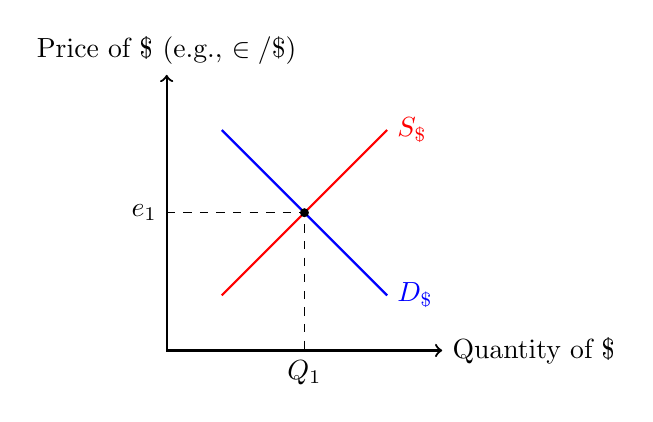
\begin{tikzpicture}[scale=0.7]
            \draw[thick,<->] (0,5) node[above]{Price of \$ (e.g., $\in / \$ $)} -- (0,0) -- (5,0) node[right]{Quantity of \$};
            \draw[thick, blue] (1,4) -- (4,1) node[right]{$D_{\$}$};
            \draw[thick, red] (1,1) -- (4,4) node[right]{$S_{\$}$};
            \draw[dashed] (0,2.5) node[left]{$e_1$} -- (2.5,2.5) -- (2.5,0) node[below]{$Q_1$};
            \filldraw (2.5,2.5) circle (2pt);
        \end{tikzpicture}
    \end{columns}
\end{frame}

% =========================================================
% SECTION 4: POLICY & ECONOMIC CONDITIONS
% =========================================================
\section{Determinants of Exchange Rates}

\begin{frame}{What Shifts Currency Supply and Demand?}
    Remember the mnemonic \textbf{T.R.I.P.S.}
    \vspace{0.5cm}
    \begin{enumerate}
        \item \textbf{T}astes and Preferences: If foreigners prefer US goods, $D_{\$} \uparrow$ (Appreciation).
        \item \textbf{R}eal Interest Rates: (Crucial for AP Exam).
        \item \textbf{I}ncome Levels: If US income rises, Americans buy more imports. $S_{\$} \uparrow$ (Depreciation).
        \item \textbf{P}rice Levels (Inflation): If US inflation is high, US goods are expensive. Exports $\downarrow$ ($D_{\$} \downarrow$) and Imports $\uparrow$ ($S_{\$} \uparrow$). Dollar depreciates.
        \item \textbf{S}peculation.
    \end{enumerate}
\end{frame}

\begin{frame}{Example: Tastes Change}
    \textbf{Scenario:} Europeans develop a strong preference for American movies.
    \begin{columns}
        \column{0.5\textwidth}
        \begin{itemize}
            \item Europeans must exchange Euros for Dollars to buy the movies.
            \item \textbf{Demand for Dollars increases.}
            \item The Dollar \textbf{Appreciates}.
            \item (Simultaneously, the supply of Euros increases in the Euro market, depreciating the Euro).
        \end{itemize}
        
        \column{0.5\textwidth}
        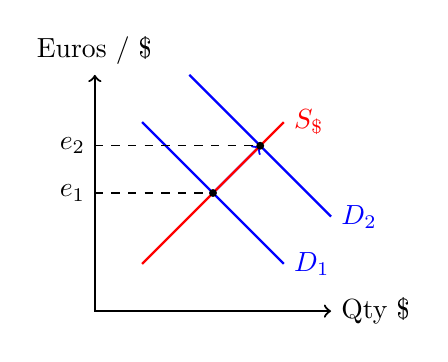
\begin{tikzpicture}[scale=0.6]
            \draw[thick,<->] (0,5) node[above]{Euros / \$} -- (0,0) -- (5,0) node[right]{Qty \$};
            \draw[thick, blue] (1,4) -- (4,1) node[right]{$D_1$};
            \draw[thick, blue, ->] (2.5,2.5) -- (3.5,3.5); % Shift arrow
            \draw[thick, blue] (2,5) -- (5,2) node[right]{$D_2$};
            \draw[thick, red] (1,1) -- (4,4) node[right]{$S_{\$}$};
            
            \draw[dashed] (0,2.5) node[left]{$e_1$} -- (2.5,2.5);
            \draw[dashed] (0,3.5) node[left]{$e_2$} -- (3.5,3.5);
            \filldraw (2.5,2.5) circle (2pt);
            \filldraw (3.5,3.5) circle (2pt);
        \end{tikzpicture}
    \end{columns}
\end{frame}

% =========================================================
% SECTION 5: REAL INTEREST RATES & CAPITAL FLOWS
% =========================================================
\section{Real Interest Rates and Capital Flows}

\begin{frame}{Interest Rates and Financial Capital}
    \begin{alertblock}{Important Concept}
        Financial capital seeks the highest Real Interest Rate ($r$).
    \end{alertblock}
    \vspace{0.3cm}
    \textbf{Scenario:} The Federal Reserve uses contractionary policy, raising US interest rates relative to Europe.
    \begin{itemize}
        \item European investors want to buy US bonds to get a higher return.
        \item \textbf{Capital Inflow} to the US increases.
        \item Demand for Dollars \textbf{increases} (foreigners need \$ to buy bonds).
        \item Supply of Dollars \textbf{decreases} (Americans keep money at home to earn high interest).
        \item \textbf{Result:} The US Dollar \textbf{Appreciates}.
    \end{itemize}
\end{frame}

% =========================================================
% SECTION 6: NET EXPORTS & FOREX
% =========================================================
\section{Net Exports and Policy}

\begin{frame}{Exchange Rates and Net Exports}
    Changes in the exchange rate affect Net Exports ($X_n$).
    \vspace{0.5cm}
    \begin{columns}
        \column{0.5\textwidth}
        \textbf{If Dollar Appreciates (Strong \$):}
        \begin{itemize}
            \item US goods look \textbf{expensive} to foreigners. Exports $\downarrow$.
            \item Foreign goods look \textbf{cheap} to Americans. Imports $\uparrow$.
            \item \textbf{Net Exports Decrease.}
        \end{itemize}
        
        \column{0.5\textwidth}
        \textbf{If Dollar Depreciates (Weak \$):}
        \begin{itemize}
            \item US goods look \textbf{cheap} to foreigners. Exports $\uparrow$.
            \item Foreign goods look \textbf{expensive} to Americans. Imports $\downarrow$.
            \item \textbf{Net Exports Increase.}
        \end{itemize}
    \end{columns}
\end{frame}

\begin{frame}{Synthesis: Fiscal Policy in an Open Economy}
    \textbf{Scenario:} Expansionary Fiscal Policy (Deficit Spending).
    \vspace{0.3cm}
    \begin{enumerate}
        \item Gov't Spending $\uparrow$ $\rightarrow$ Budget Deficit.
        \item Gov't demands loanable funds $\rightarrow$ \textbf{Real Interest Rate ($r$) $\uparrow$}.
        \item Higher $r$ attracts foreign investment (Capital Inflow).
        \item Demand for Dollars $\uparrow$ $\rightarrow$ \textbf{Dollar Appreciates}.
        \item Strong Dollar $\rightarrow$ Exports $\downarrow$, Imports $\uparrow$.
        \item \textbf{Net Exports $\downarrow$}.
    \end{enumerate}
    \vspace{0.3cm}
    \textit{Note: The decrease in Net Exports partially offsets the expansionary policy (Crowding Out via Trade).}
\end{frame}

\begin{frame}{Synthesis: Monetary Policy in an Open Economy}
    \textbf{Scenario:} Expansionary Monetary Policy (Buying Bonds).
    \vspace{0.3cm}
    \begin{enumerate}
        \item Money Supply $\uparrow$ $\rightarrow$ \textbf{Nominal Interest Rate ($i$) $\downarrow$}.
        \item Lower $i$ makes US assets less attractive (Capital Outflow).
        \item Demand for Dollars $\downarrow$, Supply of Dollars $\uparrow$.
        \item \textbf{Dollar Depreciates}.
        \item Weak Dollar $\rightarrow$ Exports $\uparrow$, Imports $\downarrow$.
        \item \textbf{Net Exports $\uparrow$}.
    \end{enumerate}
    \vspace{0.3cm}
    \textit{Note: The increase in Net Exports reinforces the expansionary policy.}
\end{frame}

\begin{frame}{Summary of Key Relationships}
    \begin{center}
    \resizebox{0.9\textwidth}{!}{
    \begin{tabular}{l c c c c c}
        \toprule
        \textbf{Event} & \textbf{Interest Rate} & \textbf{Capital Flow} & \textbf{Currency Value} & \textbf{Net Exports} \\
        \midrule
        Expansionary Fiscal & $\uparrow$ & Inflow & Appreciate & $\downarrow$ \\ 
        Contractionary Fiscal & $\downarrow$ & Outflow & Depreciate & $\uparrow$ \\ 
        Expansionary Monetary & $\downarrow$ & Outflow & Depreciate & $\uparrow$ \\ 
        Contractionary Monetary & $\uparrow$ & Inflow & Appreciate & $\downarrow$ \\ 
        \bottomrule
    \end{tabular}
    }
    \end{center}
\end{frame}

\end{document}
